\documentclass[a4paper]{llncs}
\usepackage{url}
\usepackage{epsfig}

\newcommand{\kw}[1]{\textsf{#1}}
\newcommand{\caduceus}{\textsc{Caduceus}}
\newcommand{\simplify}{\textsc{Simplify}}
\newcommand{\ergo}{\textsc{Ergo}}
\newcommand{\yices}{\textsc{Yices}}
\newcommand{\coq}{\textsc{Coq}}
\newcommand{\minelt}[1]{\ensuremath{\mathit{min\_elt}(#1)}}

\begin{document}

\title{Queens on a Chessboard: \\
       an Exercise in Program Verification}
\author{Jean-Christophe Filli\^atre}
\institute{CNRS -- Universit\'e Paris Sud \\ 91405 Orsay, France}
\maketitle

\begin{abstract}
  This article details the formal verification of a 2-lines C program
  which computes the number of solutions to the $N$-queens problem.
  The formal proof is performed using the \caduceus\ tool to generate
  the verification conditions and several provers (Simplify, Ergo,
  Coq) to discharge them. The main purpose of this article is to show
  how a complex behavior of a C program can be established with
  \caduceus. The key is here the possibility to introduce an abstract
  model and to relate it to the source code using ghost statements.
\end{abstract}

\section{Introduction}

Formal methods deal either with small properties of big programs or
big properties of small programs. This paper describes a case study
which definitely belongs to the latter category.
Indeed, it details the formal verification of the following 2-lines C program:
{\small%
\begin{verbatim}
t(a,b,c){int d=0,e=a&~b&~c,f=1;if(a)for(f=0;d=(e-=d)&-e;f+=t(a-d,(b+d)*2,(
c+d)/2));return f;}main(q){scanf("%d",&q);printf("%d\n",t(~(~0<<q),0,0));}
\end{verbatim}}
\noindent 
This rather obfuscated code was found on a web page gathering C signature
programs\footnote{\url{http://www.iwriteiam.nl/SigProgC.html}} and is
apparently due to Marcel van Kervinc. This is a standalone C program
which reads an integer on the standard input, say $n$, and then prints another
integer on the standard output, say $f(n)$. If $n$ is smaller than the
machine word size (typically 32), then
$f(n)$ appears to be the number of solutions to the famous $n$-queens
problem, that is the number of ways to put $n$ queens on a $n\times n$
chessboard so that they cannot attack each other. And even more
surprisingly, this is a very efficient program to compute this number.

As a case study for \caduceus, a tool we are
co-developing~\cite{caduceus}, we considered 
the formal verification of this program. By verification, we mean here
the mechanically-assisted proof that this program (1) does not crash, 
(2) terminates, and (3) indeed computes the expected number. 
We find this challenging to formally prove, with the highest
possible trust level, that this very low level, highly optimized
idiomatic C source code, satisfies a high level behavioral property.
% We find this
% challenging since these two lines of code are at the same time idiomatic C
% programming, complex from an algorithmic point of view and highly
% efficient. And we can demonstrate the ability of our tools to tackle
% a wide range of verification issues without considering a too long
% program. 

This paper is organized as follows. First Section~\ref{unobf}
``unobfuscates'' the program, unravelling the mystery of its algorithm
and data. Then Section~\ref{caduceus} briefly introduces \caduceus, a
tool which takes annotated C source code as input and produces
verification conditions in the native syntax of several existing provers.
Finally Section~\ref{verif} details the formal verification, namely
the logical annotations inserted in the program and the methods used
to discharge the resulting verification conditions.  The annotated
source code and the proofs are available online at
\url{http://why.lri.fr/queens/}.


\section{Unobfuscation}\label{unobf}

Before entering the formal verification process, we first unravel the
mystery behind this obfuscated code. The code is composed of two
parts: a recursive function \texttt{t}, which takes three integers as
arguments and returns an integer; and a main function which reads an
integer from the standard input, makes a call to the function
\texttt{t} and prints the result on the standard output.
With type declarations and a bit of indentation, the function
\texttt{t} reads as follows:
\begin{verbatim}
int t(int a, int b, int c) {
  int d=0,e=a&~b&~c,f=1;
  if(a) for(f=0;d=(e-=d)&-e;f+=t(a-d,(b+d)*2,(c+d)/2));
  return f;
}
\end{verbatim}
The assignment \verb!d=(e-=d)&-e! actually does not conform with the
ANSI norm, because it assumes that the inner assignment \verb!e-=d! is
performed before the evaluation of \verb!-e!. This is not guaranteed
and the compiler may freely choose between the two possible evaluation
strategies. Since \caduceus\ only deals with ANSI C programs,
we need to modify the code. Fortunately, this is quite easy:
since \verb!d! is initialized to 0 we can move the
assignment \verb!e-=d! to the end of the loop body and save the
initialization. We have even reduced the size of the original code.
The second modification we make is to replace the \texttt{main}
function with a \texttt{queens} function from \texttt{int} to
\texttt{int}, since we are only interested in the computed function
and not in input-outputs.
We end up with the code given in Figure~\ref{fig:code}. Our goal is
to show that $\mathtt{queens}(n)$ is indeed the number of
solutions to the $n$-queens problem.
\begin{figure}[t]
  \centering\hrulefill\vspace{-1em}
\begin{verbatim}
int t(int a, int b, int c) {
  int d, e=a&~b&~c, f=1;
  if (a)
    for (f=0; d=e&-e; e-=d)
      f += t(a-d,(b+d)*2,(c+d)/2));
  return f;
}
int queens(int n) {
  return t(~(~0<<n),0,0);
}
\end{verbatim}  
\vspace{-1.2em}\hrulefill\vspace{-1em}
  \caption{The C code to be verified}
  \label{fig:code}
\end{figure}

We first unravel the mystery behind the program's algorithm and data.
This is a backtracking algorithm
which fills the rows of the chessboard one at a time.
%--- there is no better way to solve the $N$-queens problem --- 
More precisely, each call to \texttt{t} enumerates all possible
positions for a queen on the current row with the \texttt{for} loop
and, for each of them, recursively calls \texttt{t} to set the next
rows.  The number of solutions is accumulated in \texttt{f} and
returned.  The key idea is the use of integers as \emph{sets} or
equivalently as \emph{bit vectors}: $i$ belongs to the ``set'' $x$ if and
only if the $i$-th bit of $x$ is set.
Following this idea, the program variables
\texttt{a}, \texttt{b}, \texttt{c}, \texttt{d} and \texttt{e} must
be seen as subsets of $\{0,1,\dots,n-1\}$.
Then almost all computations in this program are actually to be
understood as set operations. Some of them are obvious: \verb!a&~b&~c!
computes the set $\mathtt{a}\backslash\mathtt{b}\backslash\mathtt{c}$,
the test \verb!if(a)! checks whether \texttt{a} is empty, etc. Other
are more subtle. For instance, \verb!e&-e! computes the smallest
element of \texttt{e} (as a singleton set). This is a 
property of the twos-complement representation, exploited in
Patricia trees~\cite{patricia} implementations in particular.
Another trick is the computation of the set
$\{0,1,\dots,\mathtt{n}-1\}$ as \verb!~(~0<<n)!. Finally,
multiplication by 2 (resp. division by 2) is used to add 1 (resp.
subtract 1) to each element of a set; we write $\mathit{succ}$ and
$\mathit{pred}$ these two 
set operations in the following. We can thus write a more
abstract version of the code which only deals with finite sets. It is
displayed in Figure~\ref{fig:abstract}.

\begin{figure}[t]
  \hrulefill\vspace{-0.2em}
{\begin{obeylines}
  \kw{int} $t$($a$, $b$, $c$) 
  ~~~~ $f$ $\leftarrow$ 1
  ~~~~ \kw{if} $a \not= \emptyset$ 
  ~~~~~~~~ $e$ $\leftarrow$ $(a \backslash  b) \backslash c$ 
  ~~~~~~~~ $f$ $\leftarrow$ 0 
  ~~~~~~~~ \kw{while} $e \not=\emptyset$ 
  ~~~~~~~~~~~~ $d$ $\leftarrow$ $\minelt{e}$ 
  ~~~~~~~~~~~~ $f$ $\leftarrow$ $f$ $+$ $t$($a\backslash \{d\}$, $\mathit{succ}(b\cup\{d\})$, $\mathit{pred}(c\cup\{d\})$) 
  ~~~~~~~~~~~~ $e$ $\leftarrow$ $e \backslash  \{d\}$ 
  ~~~~ \kw{return} $f$ 
  ~~~~ 
  \kw{int} \textit{queens}($n$) 
  ~~~~ \kw{return} $t$($\{0,1,\dots,n-1\}$, $\emptyset$, $\emptyset$)
\end{obeylines}}
\vspace{-0.6em}\hrulefill\vspace{-1em}
  \caption{Abstract version of the code}
  \label{fig:abstract}
\end{figure}

It is now easier to explain the algorithm. The set $a$ contains the
columns not yet assigned to a queen, thus the candidate positions
for the queen to be set on the current row. Initially, $a$ contains
all possible positions, that is  $a = \{0,1,\dots,n-1\}$. 
We have found one solution whenever $a$ becomes empty and then we return 1.
Otherwise, we have to consider all possible positions on the current
row. The sets $b$ and $c$ respectively contain the positions which
must be avoided because they are on an ascending (resp. descending)
diagonal of a queen on a previous row.
Thus $e = a\backslash b\backslash c$ precisely contain the positions to be
considered for the current row. They are all examined one at a time by
repeatedly removing the smallest element from $e$, which is set to $d$.
Then the next rows are considered by a recursive call to $t$ with $a$,
$b$ and $c$ being updated according to the choice of the column $d$
for the current row: $d$ is removed from the set of possible columns
($a\backslash\{d\}$), added to the set of ascending diagonals which is
shifted ($\mathit{succ}(b\cup\{d\})$, and similarly  added to the set of
descending diagonals which is shifted the other way
($\mathit{pred}(c\cup\{d\})$). 
The values of $a$, $b$ and $c$ are illustrated in Figure~\ref{fig:abc}
for $n=8$ and 3 rows already set.

\begin{figure}
  \hspace*{-3em}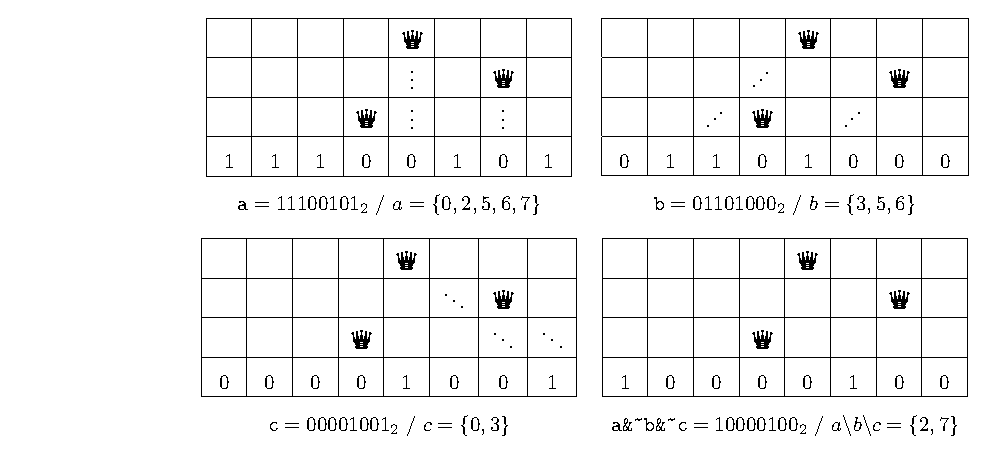
\psfig{file=figabc.eps,width=\textwidth}
  \caption{Interpretation of $a$, $b$ and $c$ as sets}
  \label{fig:abc}
\end{figure}

\section{Overview of Caduceus}\label{caduceus}

\caduceus~\cite{caduceus,FilliatreMarche04} is a tool for the
formal verification of C programs at the source code level.
The properties that may be checked are of two kinds: first, the
program may be checked to be free of threats (null pointer
dereferencing or out-of-bounds array access) and second, it may be
proved to satisfy functional properties given as annotations in the
source. These annotations include functions's preconditions and
postconditions, global invariants, loop invariants, etc., as usual in
Hoare logic frameworks~\cite{Hoare69}.
They are inserted in the source as comments of
a specific shape \texttt{/*@...*/} and written in a first-order specification
language largely inspired by the Java Modeling Language~\cite{JML}.
A significant part of ANSI C is supported, including pointer
arithmetic and possible pointer aliasing.

Here is for instance a possible specification for a function
\texttt{math\_mod} computing the modulo:
\begin{verbatim}
/*@ requires 
  @   x >= 0 && y > 0
  @ ensures 
  @   0 <= \result < y &&
  @   \exists int d; x == d * y + \result
  @*/
int math_mod(int x, int y) { ... }
\end{verbatim}
The keyword \texttt{requires} introduces the function's precondition,
that is a property to be satisfied whenever the function is called.
The keyword \texttt{ensures} introduces the function's postcondition,
that is a property which must be established whenever the function returns.
As one can notice, the specification language augments the usual
C syntax (\verb!&&!, \verb!==!, etc.) with new constructs such as
\verb!\result! denoting the value returned by the function, the
existential quantifier \verb!\exists!, etc.

Once a C source code is adequately annotated, \caduceus\
produces verification conditions. These are logical statements
expressing that the code is free of threats and fulfills the given
specification. The verification conditions are then discharged using a
general purpose theorem prover. A key feature of \caduceus\ is
its independence with respect to the prover. It indeed supports a wide
panel of existing provers, ranging from interactive proof assistants
such as \coq~\cite{coq}, PVS~\cite{PVS} or
\textsc{Isabelle/HOL}~\cite{Isabelle} to 
automatic theorem provers such as 
\simplify~\cite{simplify}, \yices~\cite{yices} or \ergo~\cite{ergo}.


\section{Formal Verification}\label{verif}

As stated in the introduction, we want to show that the C program in
Figure~\ref{fig:code} is correct using \caduceus. More precisely, we
are going to show that (1) the program does not crash; (2)
it terminates; and (3) it computes the right number.
The first property is easily obtained, since the program is not using
pointers or arrays. Thus the only threat in the code is the division and
\caduceus\ produces the corresponding verification condition $2\not=0$
which is trivially discharged. The other two properties are much more
difficult to establish.

\subsection{Integers Modelling Finite Sets}

As we explained in Section~\ref{unobf}, the program mainly uses integers
as bit vectors, to represent finite sets.  So we first start with an
axiomatization of finite sets of integers and then we make connections
between C integers and these abstract sets. It is important to say
here that we use \caduceus\ in a mode where integer overflows are not
taken into account: it means that program integers are modeled by arbitrary
precision integers. This particular point is discussed in
Section~\ref{conclu}. 

\subsubsection{Abstract finite sets.}
We introduce an abstract data type \texttt{iset} for finite sets of
integers with the following \caduceus\ declaration:
\begin{verbatim}
//@ type iset
\end{verbatim}
It is a purely logical data type which is axiomatized through a set of
constants, function symbols, predicates and axioms. We give here a small 
excerpt of this axiomatization. It is based on a
membership predicate  introduced as follows:
\begin{verbatim}
//@ predicate in_(int x, iset s)
\end{verbatim}
This is an abstract predicate, without definition. Then we can introduce
the various set operations. For instance, the empty set is introduced
with the following two declarations:
\begin{verbatim}
//@ logic iset empty()
//@ axiom empty_def : \forall int i; !in_(i,empty())
\end{verbatim}
Similarly we introduce set inclusion (\texttt{included}), cardinal
(\texttt{card}), addition and removal
of one element (\texttt{add} and 
\texttt{remove}), set difference (\texttt{diff}), smallest element
(\texttt{min\_elt}) and the \texttt{succ} and \texttt{pred} operations.
This axiomatization is 66 lines long and could obviously be a 
\caduceus\ library.

\subsubsection{C integers as finite sets.}
Next we make the connection between C operations over integers and
abstract sets. This is introduced by an abstract function symbol
\texttt{iset}, which maps a C integer to the finite set it represents:
\begin{verbatim}
//@ logic iset iset(int x)
\end{verbatim}
It is not given any definition. Indeed, we simply need to 
add axioms to interpret the C operations as set operations.
Here is one example:
\begin{verbatim}
/*@ axiom iset_c_min_elt :
  @   \forall int x; x != 0 =>
  @      iset(x&-x) == singleton(min_elt(iset(x)))
  @*/
\end{verbatim}
This new axiomatization is 30 lines long. Again it could be part of some
\caduceus\ library.

\subsection{Termination}

We now start the verification process itself by showing that the
program terminates. This is some kind of a warmup before the
correctness verification of Section~\ref{correctness}.

\subsubsection{Termination of the \texttt{for} loop.}
The termination of the \texttt{for} loop is easy to prove.
Since we are removing elements from \texttt{e} one by one until it
empties, the cardinal of \texttt{e} is the obvious variant for this
loop. It is declared with the following annotation:
\begin{verbatim}
    /*@ variant card(iset(e)) */
    for (f=0; d=e&-e; e-=d) f+=t(a-d,(b+d)*2,(c+d)/2);
\end{verbatim}
Two verification conditions are generated: one to ensure that the
variant is nonnegative and another one to ensure that the variant
decreases at each run of the loop body. Both are automatically
discharged by \simplify.

\subsubsection{Termination of the recursive function.}
Proving the termination of the recursive function \texttt{t} is more
tricky. There is also an obvious variant, namely the cardinal of
\texttt{a}, but showing that it decreases is not as easy as in the
previous case. First \caduceus\ does not support variants for
recursive functions and thus we have to introduce the corresponding
assertion manually, right before the recursive call:
\begin{verbatim}
    for (f=0; d=e&-e; e-=d) {
      //@ assert card(iset(a-d)) < card(iset(a))
      f+=t2(a-d,(b+d)*2,(c+d)/2); 
    }
\end{verbatim}
Two verification conditions are generated. 
Unfortunately they cannot be discharged automatically, because there
is some information missing. Indeed we must be able to prove that
\texttt{d} belongs to the set \texttt{a} for the cardinal to decrease,
and this is not immediate. To get this property we need the invariant
that the set \texttt{e} remains included in its initial value, which
is itself trivially included in \texttt{a}. For that purpose we
introduce the following loop invariant:
\begin{verbatim}
  //@ label L
  if (a)
    /*@ invariant included(iset(e),\at(iset(e),L)) */
    for (f=0; d=e&-e; e-=d) {
\end{verbatim}
where the label \texttt{L} is used to denote the value of
\verb!iset(e)! before entering the loop, as \verb!\at(iset(e),L)!.
Then all verification conditions are automatically discharged by \simplify.

\subsection{Correctness}\label{correctness}

We now enter the process of verifying the correctness of the program,
i.e. the property that it computes the right number of solutions. As
we have seen, the program is building the solutions one by one. Thus
we need to prove that it finds \emph{all} solutions, \emph{only}
solutions and that it does \emph{not find twice} the same
solution. There is here a major difficulty: the program is not storing
anything, not even the current solution being built. So how can we
state properties about the solutions being found? 

\subsubsection{Ghost code.} The solution is to
use \emph{ghost code}, that is additional code which is not
participating to the program computation but which can access the
program data. We first introduce ghost global variables to record the 
current solution being built:
\begin{verbatim}
//@ ghost int* col;
//@ ghost int k;
\end{verbatim}
The ghost variable \texttt{k} is the next row to be set and the ghost
array \texttt{col} records the columns assigned to the queens on the
various rows. Similarly we introduce ghost variables to store the list of
all solutions we have found so far:
\begin{verbatim}
//@ ghost int** sol;
//@ ghost int s;
\end{verbatim}
The ghost array \texttt{sol} contains all the solutions, each
solution begin an array similar to \texttt{col}.
And the ghost variable \texttt{s} is the next empty slot in \texttt{sol}. 
Using these four ghost variables, we can instrument the program with
ghost code to record the solutions:
\begin{verbatim}
int t(int a, int b, int c){
  int d, e=a&~b&~c, f=1;
  if (a)
    for (f=0; d=e&-e; e-=d) {
      //@ ghost col[k]=min_elt(d);
      //@ ghost k++;
      f += t(a-d, (b+d)*2, (c+d)/2);
      //@ ghost k--;
    }
  else 
    //@ ghost store_solution();
  return f;
}
\end{verbatim}
The particular comment \verb!//@ ghost! introduces a ghost statement,
which is similar to a traditional C statement, but may only modify
ghost variables and does not generate verification conditions
regarding pointers validity (ghost arrays are infinite).
The function \texttt{store\_solution} is a ghost
function\footnote{There is not yet a notion of ghost function in
  \caduceus\ so we use a usual C prototype; it is thus our
  responsibility to check that it is not called in the normal code,
  which is here obvious.} that we introduce to record a solution when
it is found and which we now describe.

\subsubsection{Solutions.}
To give \texttt{store\_solution} a specification, we need to introduce
the notion of solution to the $N$-queens problems. It is convenient to
introduce the size of the chessboard as a logical constant:
\begin{verbatim}
//@ logic int N()
\end{verbatim}
It is also convenient to start defining the more general notion of
\emph{partial solution}, for the first $k$ rows:
\begin{verbatim}
/*@ predicate partial_solution(int k, int* s) {
  @   \forall int i; 0 <= i < k => 
  @     0 <= s[i] < N() &&
  @     (\forall int j; 0 <= j < i => s[i] != s[j] &&
  @                                   s[i]-s[j] != i-j &&
  @                                   s[i]-s[j] != j-i)
  @ } */
\end{verbatim}
$\mathtt{partial\_solution}(k,s)$ states that the array $s$ contains
column assignments for the first $k$ queens on the first $k$
rows. Each column $s[i]$ must be in the valid range $[0,N[$ and two
queens on two different rows $i$ and $j$ may not attack each other.
Then we can define the notion of solution, as a partial solution for
the $N$ rows:
\begin{verbatim}
//@ predicate solution(int* s) { partial_solution(N(), s) }
\end{verbatim}
We also introduce two handy predicates \texttt{eq\_prefix} and
\texttt{eq\_sol} to state that two solutions coincide up a given row:
\begin{verbatim}
/*@ predicate eq_prefix(int *t, int *u, int i) {
  @   \forall int k; 0 <= k < i => t[k]==u[k]
  @ } */
//@ predicate eq_sol(int *t, int *u) { eq_prefix(t, u, N()) } 
\end{verbatim}
Finally we can give \texttt{store\_solution} a specification:
\begin{verbatim}
/*@ requires solution(col)
  @ assigns  s, sol[s][0..N()-1]
  @ ensures  s==\old(s)+1 && eq_sol(sol[\old(s)], col)
  @*/
void store_solution();
\end{verbatim}
It has a precondition which enforces the user to show that
\texttt{col} contains a valid solution, an \texttt{assigns} clause
specifying that it only modifies \texttt{s} and the \texttt{s}-th row
of \texttt{sol}, and a postcondition ensuring that \texttt{s} has been
incremented and \texttt{col} stored in \verb!sol[s]!.
With this precondition, \texttt{store\_solution} already ensures that
we find only solutions. We still need to show that we find \emph{all}
solutions, without duplicates.

\subsubsection{All solutions, without duplicates.}
To ensure that we find all solutions, we give \texttt{queens} the
following postcondition:
\begin{verbatim}
/*@ ensures 
  @   sorted(sol,0,s) &&
  @   \forall int* t; solution(t) 
  @     <=> (\exists int i; 0<=i<\result && eq_sol(t,sol[i]))
  @*/
int queens(int n);
\end{verbatim}
In other words, an array is a solution if and only if it appears in
\texttt{sol} when we are done, and moreover \texttt{sol} is a sorted
array so it does not contain duplicated solutions. To define the
\texttt{sorted} predicate, we introduce a natural lexicographic order
over solutions, as follows:
\begin{verbatim}
/*@ predicate lt_sol(int *s1, int *s2) {
  @   \exists int i; 0<=i<N() && eq_prefix(s1,s2,i) && s1[i]<s2[i]
  @ } */
/*@ predicate sorted(int **s, int a, int b) {
  @   \forall int i, int j; a <= i < j < b => lt_sol(s[i], s[j])
  @ } */
\end{verbatim}

\subsubsection{Remaining annotations.} 
We are now done with the annotations ensuring the correctness of the
program. But to establish the verification conditions, we still need
to give \texttt{t} a specification and its loop an invariant. The
fully annotated code is given in appendix. Here are the key properties
stated in these annotations:
\begin{itemize}
\item The precondition of \texttt{t} requires that \texttt{col} must be a
  partial solution up to row $k$, and that \texttt{a},
  \texttt{b} and \texttt{c} are consistent with \texttt{col}, as
  explained in Section~\ref{unobf}.
\item The postcondition of \texttt{t} ensures that the set of
  solutions built by \texttt{t} is sorted and contains exactly the 
  solutions extending the partial solution given at the entry point.
\item The loop invariant states that \texttt{sol} remains sorted and
  that the set of solutions built since the beginning of the loop are
  exactly those extending the partial solution given at the entry
  point of \texttt{t} with a column for the row $k$ taken among the
  elements of $e$ already considered by the \texttt{for} loop.
\end{itemize}
We end up with 46 lines of annotations (not including the preliminary
definitions and axiomatizations!) for 2 lines of code. This huge
ratio must be considered as extreme: we are proving a very complex
property of a very complex and very small code. This is obviously not
the case in all formal verifications.

\subsubsection{Discharging the verification conditions.}
When \caduceus\ is run on the resulting annotated source code, we get
57 verification conditions for \texttt{t} and 16 for
\texttt{queens}. Regarding the latter, all verification conditions are
automatically discharged by \simplify, within a few seconds.
Regarding the former, only 44 verification conditions are
automatically discharged, either by \simplify\ or \ergo.
The remaining 13 verification conditions were discharged manually,
using the \coq\ proof assistant, but with the help of the ATPs
\simplify\ and \ergo\ called from \coq\ on some subgoals. These \coq\
proof scripts amount to 600 lines and represent several hours of
work. Though these tools could be better integrated, this
collaboration between interactive and automatic provers can be
considered successful.

\section{Conclusion}\label{conclu}

We have presented the formal verification of an extremely short but
also extremely complex C program using the \caduceus\ tool. Beyond a
nice specification exercise, it was the opportunity to illustrate
several key features of \caduceus:
\begin{itemize}
\item 
  First, \caduceus\ allows the user to introduce arbitrary
  \emph{first-order logical theories} for the purpose of the
  specification. This includes types, constants, functions, predicates
  and axioms, all declared within the program source code and passed
  to the provers used to discharge the verification conditions.
  We consider this ability as a real improvement with respect to
  JML-like approaches~\cite{JML} where annotations may only refer to code data
  and (pure) code functions. 

\item 
  Second, this case study clearly points out the necessity of
  \emph{ghost code} to write specifications. In this particular case,
  the program is enumerating the solutions to a problem, but is not
  storing any of them, not even the current one. Thus the code has to
  be enriched with new statements ``to tell the untold'' and thus to
  enable the specification. In particular, ghost code must not be
  limited to mere assignments but should include arbitrary statements,
  up to function calls. The support of ghost code in \caduceus\ was
  not optimal in this respect; we plan to extend it accordingly.

\item 
  Finally, the large set of verification conditions could be
  discharged using the collaborative work of three automatic provers
  (\simplify, \ergo\ and \yices) and an interactive proof assistant
  (\coq). This multi-provers architecture is one of the main features
  of \caduceus\ and has been emphasized since the
  beginning~\cite{FilliatreMarche04}. Obviously, the proof could not
  have been conducted using automatic provers only and would have been
  a tremendous amount of work as a fully interactive proof.
\end{itemize}

There is a remaining unsatisfactory aspect in this formal
verification which deserves discussion: \emph{integer
overflows}. Indeed, the verification was performed in a model where C
integers are mapped to mathematical integers and not to 32-bits
machine integers (assuming a 32-bits architecture). The limitation
$n\le 32$ is not really an issue, the world record holding for $n=25$;
thus all machines will be 64-bits before the limit $n=32$ is reached.
But the program is actually performing unrelevant overflows as soon as
$n>16$. Thus for the verification to be fully satisfactory, it should
be conducted within a model where we can prove that the $n$ lowest
bits only of the program variables are meaningful. But such a model
should not penalize the work of automatic provers, which all assume
mathematical integers. Regarding \caduceus, this is ongoing research.

\nocite{*}
\bibliographystyle{plain}
\bibliography{./biblio}

\appendix
\section{Annotated Source Code}\label{app:code}
{\footnotesize
\begin{verbatim}
/*@ requires
  @   0 <= k && k + card(iset(a)) == N() && 0 <= s &&
  @   pre_a:: (\forall int i; in_(i,iset(a)) <=> 
  @            (0<=i<N() && \forall int j; 0<=j<k => i != col[j])) &&
  @   pre_b:: (\forall int i; i>=0 => (in_(i,iset(b)) <=> 
  @            (\exists int j; 0<=j<k && col[j] == i+j-k))) &&
  @   pre_c:: (\forall int i; i>=0 => (in_(i,iset(c)) <=> 
  @            (\exists int j; 0<=j<k && col[j] == i+k-j))) &&
  @   partial_solution(k, col)
  @ assigns
  @   col[k..], s, k, sol[s..][..]
  @ ensures  
  @   \result == s - \old(s) && \result >= 0 && k == \old(k) &&
  @   sorted(sol, \old(s), s) &&
  @   \forall int* t; ((solution(t) && eq_prefix(col,t,k)) <=>
  @                    (\exists int i; \old(s)<=i<s && eq_sol(t, sol[i])))
  @*/
int t(int a, int b, int c){
  int d, e=a&~b&~c, f=1;
  //@ label L
  if (a)
    /*@ invariant 
      @   included(iset(e),\at(iset(e),L)) &&
      @   f == s - \at(s,L) && f >= 0 && k == \old(k) && 
      @   partial_solution(k, col) &&
      @   sorted(sol, \at(s,L), s) &&
      @   \forall int *t; 
      @     (solution(t) && 
      @      \exists int di; in_(di, diff(\at(iset(e),L), iset(e))) &&
      @          eq_prefix(col,t,k) && t[k]==di) <=>
      @     (\exists int i; \at(s,L)<=i<s && eq_sol(t, sol[i]))
      @ loop_assigns
      @   col[k..], s, k, sol[s..][..]
      @*/
    for (f=0; d=e&-e; e-=d) {
      //@ assert \exists int x; iset(d) == singleton(x) && in_(x,iset(a)) 
      //@ ghost col[k] = min_elt(d);
      //@ ghost k++;                
      f += t(a-d, (b+d)*2, (c+d)/2);
      //@ ghost k--;                
    }
  else 
    //@ ghost store_solution();
  return f;
}

/*@ requires 
  @   n == N() && s == 0 && k == 0
  @ ensures 
  @   \result == s &&
  @   sorted(sol, 0, s) &&
  @   \forall int* t; 
  @      solution(t) <=> (\exists int i; 0<=i<\result && eq_sol(t,sol[i]))
  @*/
int queens(int n) {
  return t(~(~0<<n),0,0);
}
\end{verbatim}
}

\end{document}
